\section{System Design}
\label{ch:system-design}

\epigraph{That men do not learn very much from the lessons of history is the most important of all the lessons that history has to teach.}{Aldous Huxley}

\subsection{System Architecture Diagram}
\begin{figure}[h]
\caption{System Architecture}
\centering
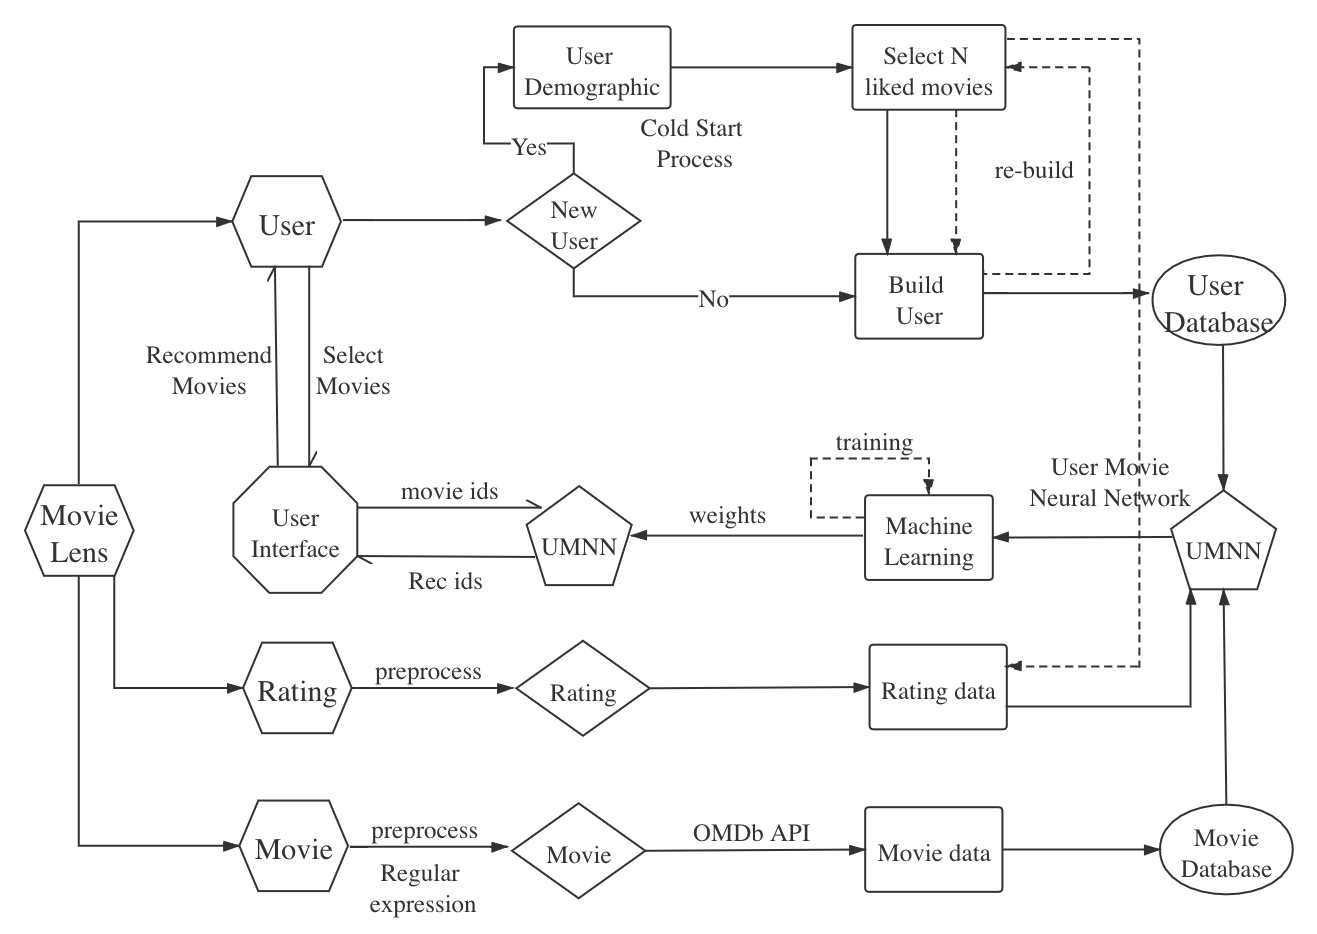
\includegraphics[width=1.0\textwidth]{system_architecture}
\end{figure}
\subsubsection{MovieLens Dataset}
%build user database and movie database
We use the MovieLens dataset from the GroupLens Research Group at the University of Minnesota. The MovieLens 1M dataset is used as the data source in this paper. It contains 1 million ratings of 4,000 movies from 6,000 users. It is divided into three tables: movie ratings, movie metadata (genre style and age), and demographic data about users (age, zip code, gender, and occupation).
\subsubsection{4 Data Tracks}
In the system architecture diagram. The two outputs from the MovieLens extract the movie table and rating table as the input of the movie module, and extract the user table as the input of the user module. The user and the movie, respectively, represent two paths, which represent the behavior trajectory when a user or a movie is entered in the system. This paper divides the entire recommendation system into four parts according to the business path, which are the user data track, movie data track, rating data track, and recommendation generation track. In the following paragraphs, we introduce each track separately.
\par In terms of user trajectory, each time a user comes in, it is necessary to determine whether the user is a new one. Once a new user is found, a cold start strategy will be initiated. The system will guide the user to enter relevant personal information (gender, age, occupation). Then take a series of top-N movies from the existing movie data and let the user choose some movies he likes. After selecting n movies (in the subsequent prototype, we set n to 10 for easy description and testing). The system will use the previously obtained personal information of the user and the selected n favorite movies as input to build a user portrait, that is, the "Build user" part in the system architecture diagram. If the user is not involved in the cold start problem, the user goes to the "Build User" process directly. This part of the user data is the existing user data obtained from the user table in MovieLens. In summary, the existing user data in MovieLens and newly entered user data constitute the entire user database of the system together.
\par There are two types of labeling for movies, which are the characteristics of the movie itself (name, genre, director, actor) and the behavior characteristics of the movie in the system.
Movie characteristics:
The properties of the movie itself do not need to be updated frequently. These data will hardly change or need to be updated after the first input into the system. The genre of the movie and its release year can be retrieved from MovieLens.
\begin{figure}[h]
\caption{UMNN Module}
\centering
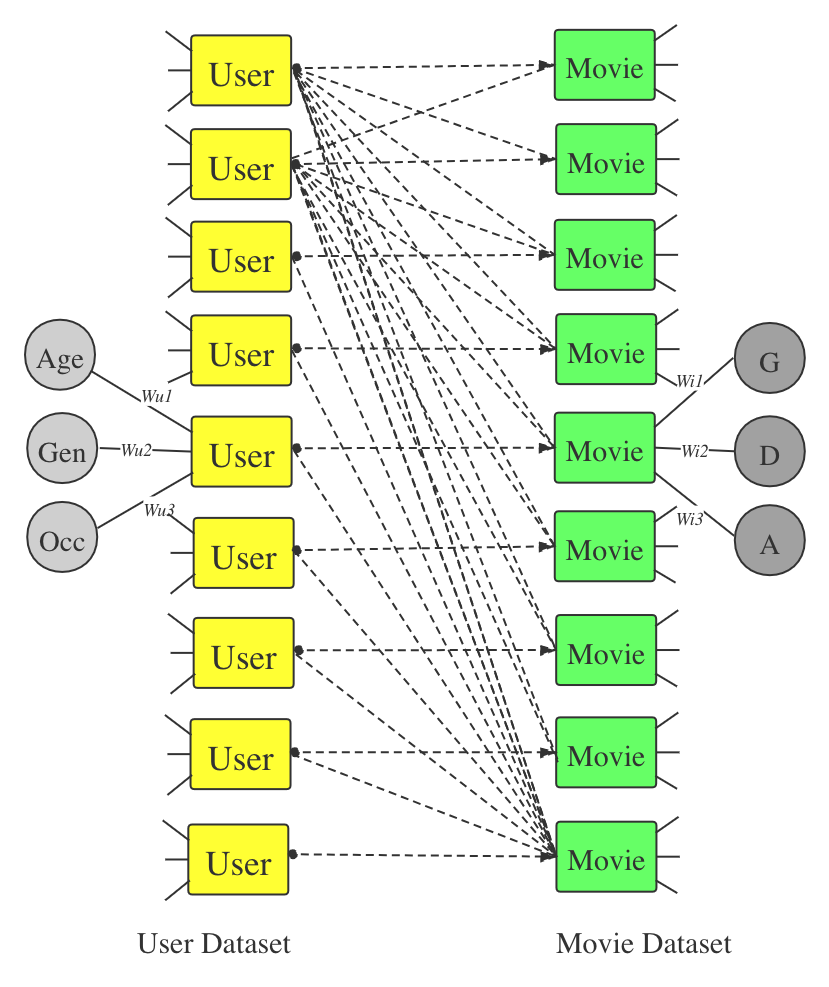
\includegraphics[width=0.5\textwidth]{UMNN_system}
\end{figure}
\par The movie data of MovieLens does not include the director, actor, writer, poster and other data of the movie. In order to obtain more useful movie metadata, so that the system we are constructing can have richer information and data to show, we use OMDb API which is a third-party RESTful web service to get movie information. The name and year of each movie are used as query inputs to obtain the director, actor, writer, and poster addresses of the movie. The new data corresponding to all movies in the entire movie table is re-integrated into a new movie table. The data items constituting the new movie table are: (iid, title, year, genre, director, actor, writer). The new movie table constitutes the "Movie Database" part in the system architecture diagram.
Movie behavior characteristics:
Movie behavior characteristics refer to information such as the movie being clicked and rated in the system.
\par When the movie and user characteristics are collected, the "Movie Database" and the "User Database" are formed. These two components can be combined to build a model training set. All data in user database and movie database are structured as shown in the figure UMNN Module. The data structure in the rating table contains someone user's rating of someone movie. The data of the rating table is used as a mapping from the user dataset to the movie dataset. All user nodes and movie nodes that are related in the rating table are connected. All connections in the user dataset and movie dataset have weight values, and their initial value is set to the user's rating of the movie. In summary, the training set UMNN in the system architecture diagram is finally molded. With some machine learning algorithms provided by pytorch, by multiple rounds of training on UMNN, a UMNN with a series of new weights after fitting is constructed. The UMNN model is used as the core module of the recommendation system. When the user selects N movies he likes in the User Interface, the User Interface sends the selected movie id list as input to the UMNN, and the UMNN sends the recommended id list to the User Interface, and the User Interface finally shows the recommended movies' Information.

\subsubsection{UMNN}
\subsubsection{Frontend and Backend}
\subsubsection{Cold Start}

\subsection{Recommendation Strategy}
\subsubsection{Recommendation Style}
\begin{itemize}

\item[(a)]\textbf{Popularity-Based}\\
There are two reasons for recommending based on popularity. First, popularity often represents the important characteristics of a product. Some users utilize extensive sources of information before making decisions to choose a movie, however, the others depend on simple and limited sources of information. But they all will be affected by the popularity of movies to some extent. Second, the popularity of a movie greatly influences user's decisions. From a psychological perspective, when recommending popular movies to users, even if they are not the type the user likes, users usually subconsciously give these movies a higher rating\cite{ahn2006utilizing}. So popularity-based recommendation is a very important and simple method in the early days. In this paper, popularity-based method is used as the basis for the other four recommendation methods.
\item[(b)]\textbf{User-Based}\\
\begin{figure}[h]
\caption{user-based recommendation strategy}
\centering
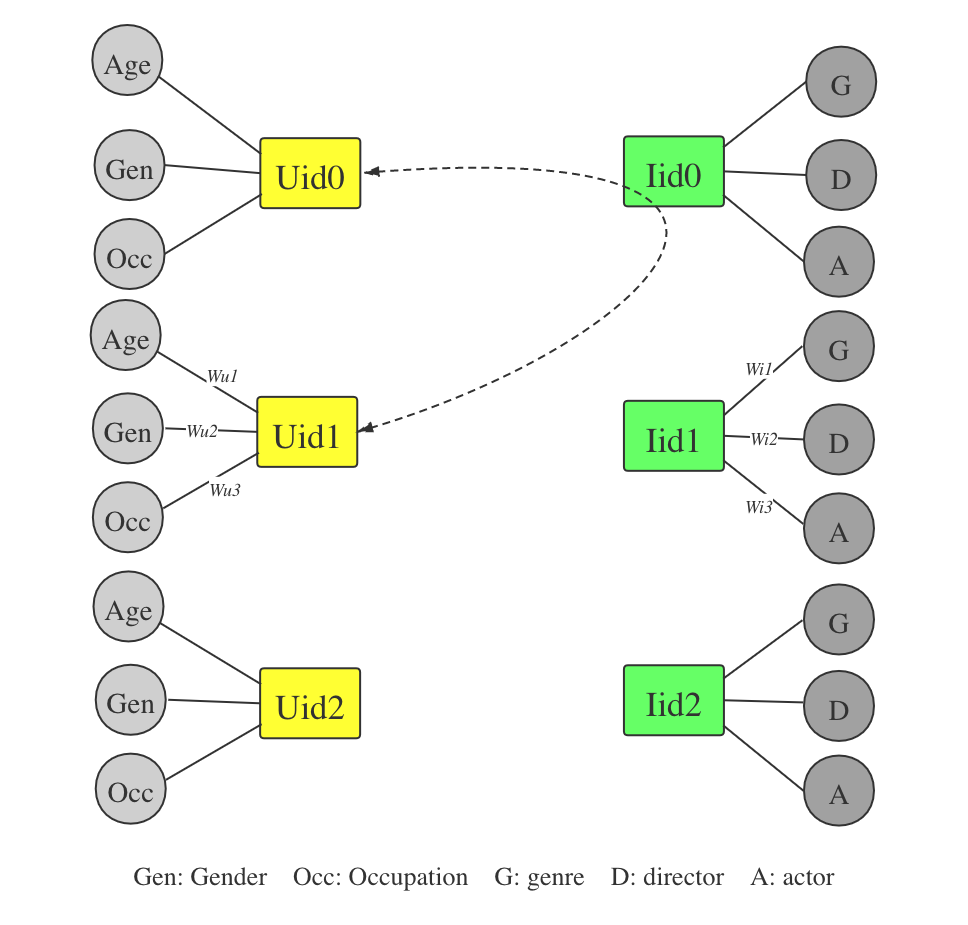
\includegraphics[width=0.5\textwidth]{neural_network_user_based}
\end{figure}
The user-based recommendation strategy more considers the interests of new user and other users with the same hobbies, recommends items that other users like / visited to the new user, and has little to do with new user's current behavior.What will be recommended to a new user, depends on what the other users have visited before. The recommended items are the favorite items of users with the same hobby, so it has a hotspot effect. it can recommend the items that the other users have just visited. It has strong real-time performance, especially the newly introduced hot spots, which can spread quickly and solve the cold start problem of new-item.
\item[(c)]\textbf{Item-Based}\\
\begin{figure}[h]
\caption{item-based recommendation strategy}
\centering
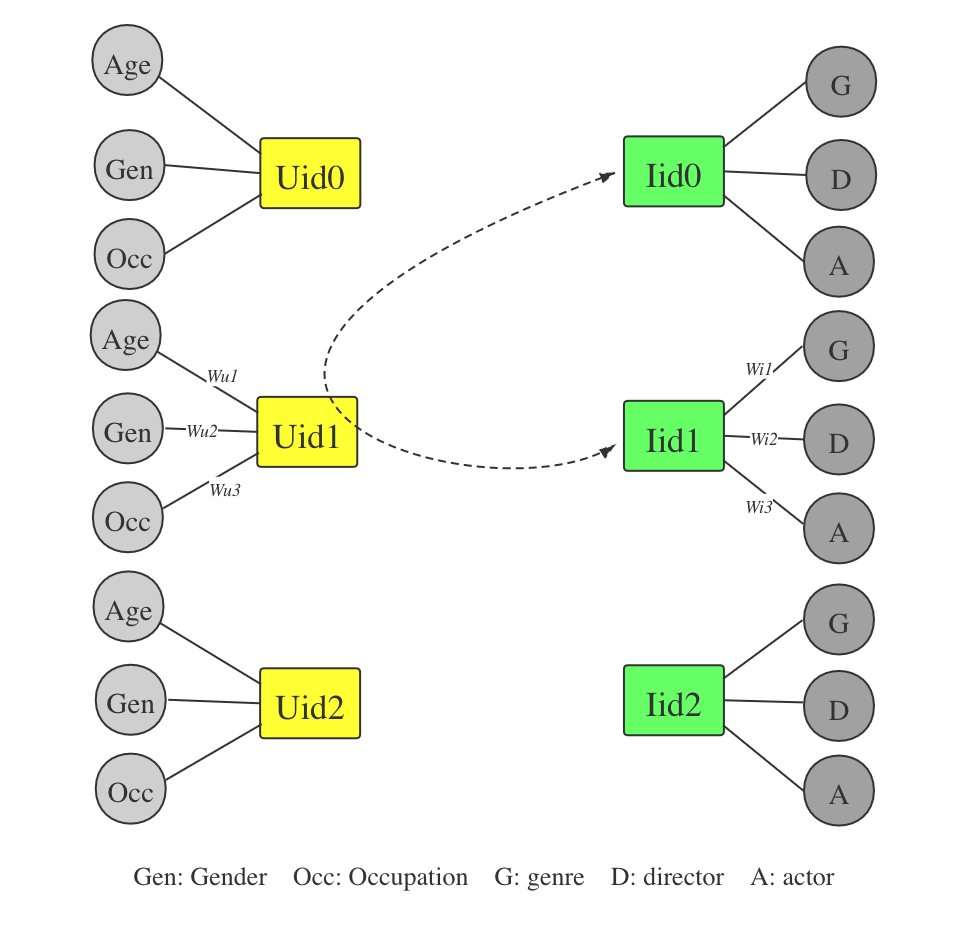
\includegraphics[width=0.5\textwidth]{neural_network_item_based}
\end{figure}
Item-based mainly uses users' historical interests to make recommendations. Recommending items that are similar to the user's history. This method has a lot to do with the user's current behavior. The similarity between the item recommended to the user and the item previously selected by the user is understandable by the user, which is called Interpretable. Most of the recommended items are not popular, but are related to the interests of users. This recommendation method has the highest accuracy when the user's interest is long-term and fixed. The significance of Item-based recommendation is to help users find items related to their interests. The recommended item is not related to user identity, so it is better to solve the problem of new users.
\par Badrul et al.\cite{sarwar2001item} compared the performance of user-based and item-based and demonstrated that the item-based algorithm provides better quality of prediction than the user-based algorithm.
\item[(d)]\textbf{Demographic-Based}\\
\begin{figure}[h]
\caption{demographic-based recommendation strategy}
\centering
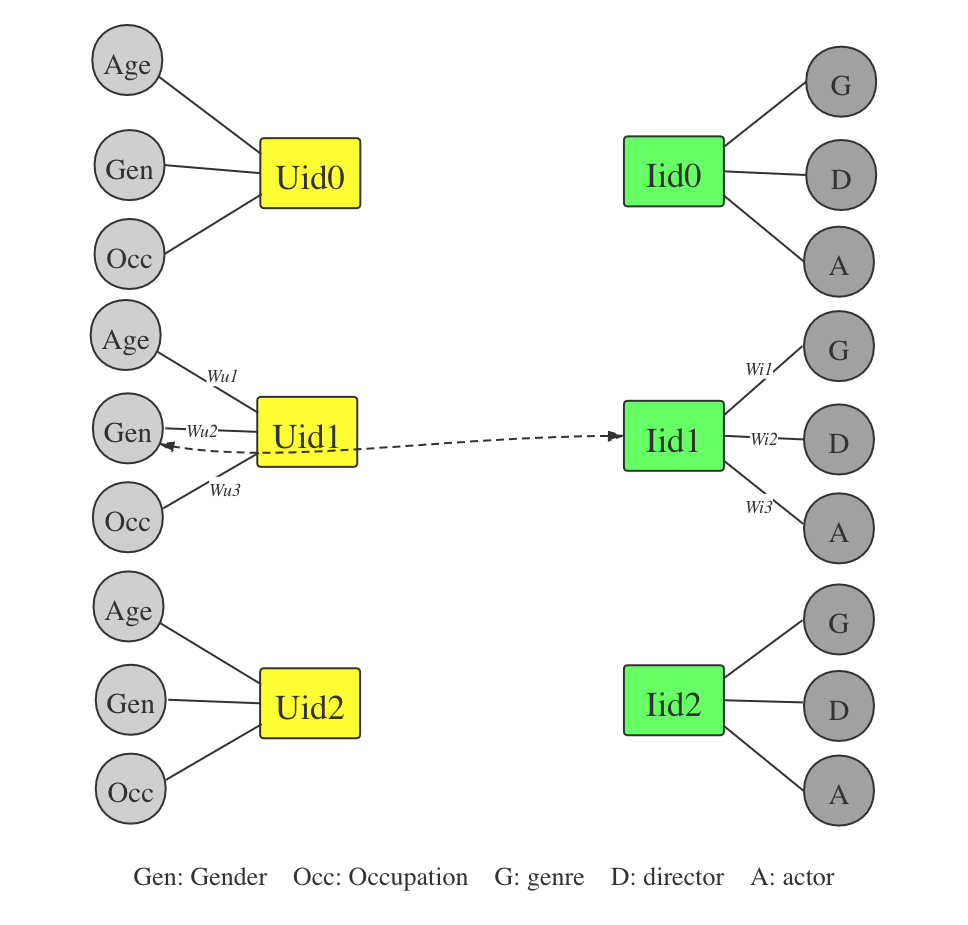
\includegraphics[width=0.5\textwidth]{neural_network_demographic_based}
\end{figure}
According to the basic information of the system user, find out the relevance of the user, and then make recommendations. At present, it is rarely used alone in large systems, and it is usually used in combination with other recommendation algorithms. The usual method is to classify the user based on the user's registration information, and then recommend to the user the items in the category to which she belongs. In this paper, we use gender, age and occupation of user as feature of demographic-based recommendation method.
\item[(e)]\textbf{Content-Based}\\
\begin{figure}[h]
\caption{content-based recommendation strategy}
\centering
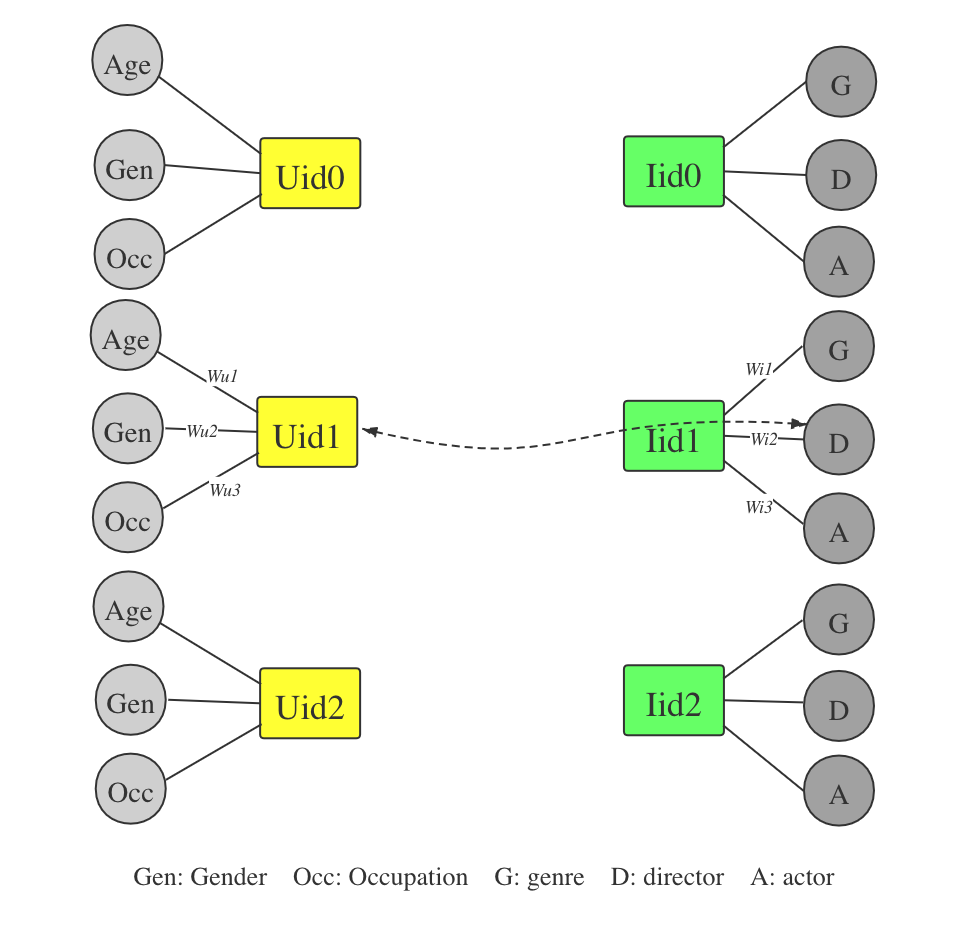
\includegraphics[width=0.5\textwidth]{neural_network_content_based}
\end{figure}
Based on the user's past browsing history, make recommendations to the user that he/she has not viewed. Recommendations are generally based on keywords or content features. For example, if a user has previously chosen to be interested in a certain director's movie, the user will be recommended with the other movie works of this director. The advantage of this method is that there is no popularity bias, items with rare features can be recommended, and user content characteristics can be used to provide recommendation explanations. The disadvantage is that the content must be machine-readable and meaningful, and the features of the recommended content need to be archived in advance.
\par Recommend movies that are similar to movies that users have liked. It is mainly based on the comparison of movie attribute information and user portrait information. The core problem is how to establish the association between movie attributes and user information. it assumes that users will rate items having alike features similarly\cite{safoury2013exploiting}.

\end{itemize}

\par For various reasons, it is easier to collect the user's past behavior than to collect user information, but CF-based (user-based and item-based) has it's limitations. When the scoring is very sparse, the prediction accuracy will be greatly reduced. And the cold start of new products is also a problem for CF. In general, therefore, most of today's recommendation systems use a hybrid recommendation method.
\subsubsection{Recommendation Explanation Strategy}
\subsubsection{Recommendation Explanation Adaptation Strategy}
%rule based

\subsection{Machine Learning Algorithm}

\subsubsection{Tool and Library}
%weights
PyTorch\cite{ketkar2017introduction} and TensorFlow\cite{abadi2016tensorflow} are currently the most popular methods for investigating deep learning and neural networks. PyTorch is more useful for researchers, enthusiasts and Individual developers to quickly build prototype in small-scale projects. TensorFlow is more suitable for large-scale deployments, especially when cross-platform and embedded deployments are required. In our research, PyTorch was selected for its vast repository of libraries to handle dataset preprocessing, statistical analysis, plotting, and more.\cite{paszke2019pytorch}.

\subsubsection{Neural Network Model}
%node and item
\subsubsection{Training Weights}


\subsection{User Interface Prototype} 

\subsubsection{Development Tool and Language}
\subsubsection{Prototype}
\subsubsection{}

\subsection{}

\cleardoublepage